
%(BEGIN_QUESTION)
% Copyright 2006, Tony R. Kuphaldt, released under the Creative Commons Attribution License (v 1.0)
% This means you may do almost anything with this work of mine, so long as you give me proper credit

A {\it horsepower} is defined as 550 ft-lbs of work done in one second of time.  An example of this would be a 550 pound weight lifted vertically at a speed of one foot per second, or a one pound weight lifted vertically at a speed of 550 feet per second.

There is a way to relate this to rotary motion, not just linear motion.  In the case of rotary motion we must deal with torque ($\tau$) in lb-ft and angular speed ($S$) in revolutions per minute (RPM) rather than force in pounds and linear speed in feet per second.

Just as linear power is proportional to the product of force and velocity ($P \propto F v$), rotary power is proportional to torque and rotary speed ($P \propto \tau S$).  What we need to turn this proportionality into an equality is a multiplying constant ($k$):

$$P = k \tau S$$

We may determine the value of this constant by setting up a ``thought experiment'' that translates between linear power and rotary power:

$$\includegraphics[width=15.5cm]{i01430x01.eps}$$

In this case, we have a 1 foot radius drum hoisting a 550 pound weight at a linear velocity of 1 foot per second, the definition of one horsepower.  Translate the linear force and linear velocity to rotary force (torque) and rotary velocity (revolutions per minute), and then calculate the necessary $k$ factor to make your own torque/speed/horsepower equation.

\underbar{file i01430}
%(END_QUESTION)





%(BEGIN_ANSWER)

The torque ($\tau$) in this case is obviously 550 lb-ft, since the 550 pound weight is acting on a moment arm 1 foot long (the drum's radius).  All we need to do is translate the vertical velocity of 1 foot per second into drum rotation in units of RPM, and we'll have the data we need to calculate $k$:

\vskip 10pt

$$\hbox{Circumference of drum } = \pi D = 2 \pi r = 6.283 \hbox{ ft}$$

This is the amount of cable that travels in one revolution of the drum (1 rev = 6.283 ft), and this equality constitutes a conversion factor which we may use to convert the linear velocity of 1 ft/s into a rotational velocity:

\vskip 10pt

$$\left({{1 \hbox{ ft}} \over \hbox{sec}} \right)  \left({{1 \hbox{ rev}} \over {6.283 \hbox{ ft}}}\right) \left( {{60 \hbox{ sec}} \over {1 \hbox{ min}}} \right) = 9.5493 \hbox{ RPM}$$

Therefore, 

$$P = k \tau S$$

$$1 \hbox{ hp}  = (k) (550 \hbox{ ft-lb}) (9.5493 \hbox{ RPM})$$

$$k = 0.0001904$$

$$P = 0.0001904 \tau S$$

$$\hbox{. . . or . . .}$$

$$P = {{\tau S} \over 5252}$$

\noindent
Where,

$P$ = Shaft power in horsepower

$\tau$ = Shaft torque in lb-ft

$S$ = Shaft speed in revolutions per minute (RPM)

\vskip 10pt

By coincidence, the factor of 5252 happens to be close to the number of feet in a mile (5280 feet = 1 mile).  This might come in handy as an approximation!

%(END_ANSWER)





%(BEGIN_NOTES)


%INDEX% Physics, torque: calculation problem
%INDEX% Physics, torque: shaft horsepower

%(END_NOTES)


